\section{液体的压强}\label{sec:5-5}

液体因为受到重力的作用,所以对容器的底要产生压强。这可以用实验来证明。
在一个玻璃管的下端,扎上一块橡皮膜,把水灌进管里,橡皮膜就向外凸出(图 \ref{fig:5-15}),表明管底受到了水的压强。
水灌得越深,橡皮膜突出得越厉害,表明管底受到的水的压强越大。

\begin{figure}[htbp]
    \centering
    \begin{minipage}{7cm}
    \centering
    \vspace{3em}
    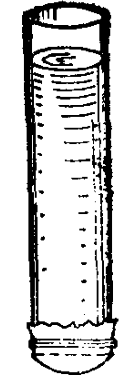
\includegraphics[width=1.75cm]{../pic/czwl1-ch5-15}
    \caption{液体对容器底有压强}\label{fig:5-15}
    \end{minipage}
    \qquad
    \begin{minipage}{7cm}
    \centering
    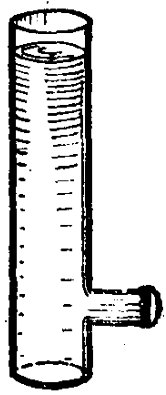
\includegraphics[width=2.5cm]{../pic/czwl1-ch5-16}
    \caption{液体对侧壁有压强}\label{fig:5-16}
    \end{minipage}
\end{figure}


取一个侧壁上开孔的圆筒,把橡皮膜扎在侧壁的孔上,向容器内灌水,可以看到,
橡皮膜也向外凸出(图 \ref{fig:5-16}),这表明水对侧壁也有压强。
如果在圆筒的不同高度处开几个小孔,向筒里灌水,可以看到水就从各个小孔喷出来,小孔越低,水喷得越急(图 \ref{fig:5-17})。
这明水对侧壁的压强是随着深度的增加而增大的。

\begin{figure}[htbp]
    \centering
    \begin{minipage}{7cm}
    \centering
    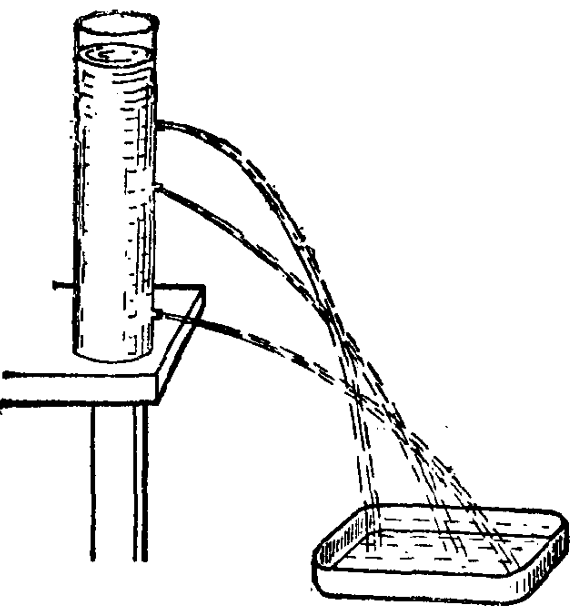
\includegraphics[width=6cm]{../pic/czwl1-ch5-17}
    \caption{液体的压强随深度而增大}\label{fig:5-17}
    \end{minipage}
    \qquad
    \begin{minipage}{7cm}
    \centering
    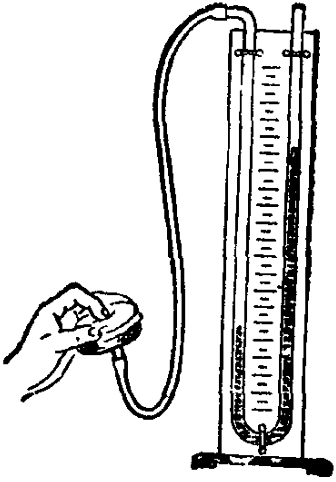
\includegraphics[width=5cm]{../pic/czwl1-ch5-18}
    \caption{压强计}\label{fig:5-18}
    \end{minipage}
\end{figure}

液体不但对容器的底和侧壁有压强,而且在液体的内部也有压强。液体内部的压强可以用压强计来测量。
图 \ref{fig:5-18} 是一个用 U 形玻璃管制成的压强计。玻璃管里装着有色的水,如果两边水面上的压强相等,两边的水面就在同一高度。
如果左管中水面上的压强增加,左管中的水面就下降,右管中的水面就上升。
从两管中水面的高度差,就可以知道两管中水面上的压强差。

用橡皮管把一个扎有橡皮膜的金属圆盒连到压强计的左管上。
用手压橡皮膜,手产生的压强使左管的水面下降,右管的水面上升。
加在橡皮模上的压强越大,两管中水面的高度差越大。

\begin{figure}[htbp]
    \centering
    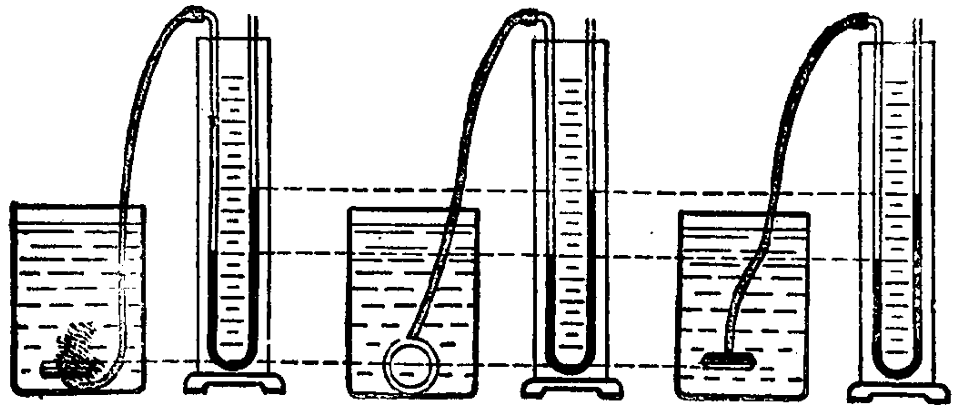
\includegraphics[width=0.6\textwidth]{../pic/czwl1-ch5-19}
    \caption{在液体内部同一深度,向各个方向的压强都相等}\label{fig:5-19}
\end{figure}

现在我们用压强计来研究液体内部的压强。
把压强计的金属盒放入液体中,可以看到,压强计两管中的水面也产生高度差。这表明液体内部也有压强。
压强计的金属盒放入液体中越深,两管中水面的高度差越大。
可是在同一深度处,不论金属盒口向上、向下、向侧或向任何方向,压强计两管中水面的高度差都相等(图 \ref{fig:5-19})。
这表明,\CJKunderwave{液体内部向各个方向都有压强,压强随深度的增加而增大,但在同一深度,液体向各个方向的压强相等}。




